\documentclass{article}[18pt]
\ProvidesPackage{format}
%Page setup
\usepackage[utf8]{inputenc}
\usepackage[margin=0.7in]{geometry}
\usepackage{parselines} 
\usepackage[english]{babel}
\usepackage{fancyhdr}
\usepackage{titlesec}
\hyphenpenalty=10000

\pagestyle{fancy}
\fancyhf{}
\rhead{Sam Robbins}
\rfoot{Page \thepage}

%Characters
\usepackage{amsmath}
\usepackage{amssymb}
\usepackage{gensymb}
\newcommand{\R}{\mathbb{R}}

%Diagrams
\usepackage{pgfplots}
\usepackage{graphicx}
\usepackage{tabularx}
\usepackage{relsize}
\pgfplotsset{width=10cm,compat=1.9}
\usepackage{float}

%Length Setting
\titlespacing\section{0pt}{14pt plus 4pt minus 2pt}{0pt plus 2pt minus 2pt}
\newlength\tindent
\setlength{\tindent}{\parindent}
\setlength{\parindent}{0pt}
\renewcommand{\indent}{\hspace*{\tindent}}

%Programming Font
\usepackage{courier}
\usepackage{listings}
\usepackage{pxfonts}

%Lists
\usepackage{enumerate}
\usepackage{enumitem}

% Networks Macro
\usepackage{tikz}


% Commands for files converted using pandoc
\providecommand{\tightlist}{%
	\setlength{\itemsep}{0pt}\setlength{\parskip}{0pt}}
\usepackage{hyperref}

% Get nice commands for floor and ceil
\usepackage{mathtools}
\DeclarePairedDelimiter{\ceil}{\lceil}{\rceil}
\DeclarePairedDelimiter{\floor}{\lfloor}{\rfloor}

% Allow itemize to go up to 20 levels deep (just change the number if you need more you madman)
\usepackage{enumitem}
\setlistdepth{20}
\renewlist{itemize}{itemize}{20}

% initially, use dots for all levels
\setlist[itemize]{label=$\cdot$}

% customize the first 3 levels
\setlist[itemize,1]{label=\textbullet}
\setlist[itemize,2]{label=--}
\setlist[itemize,3]{label=*}

% Definition and Important Stuff
% Important stuff
\usepackage[framemethod=TikZ]{mdframed}

\newcounter{theo}[section]\setcounter{theo}{0}
\renewcommand{\thetheo}{\arabic{section}.\arabic{theo}}
\newenvironment{important}[1][]{%
	\refstepcounter{theo}%
	\ifstrempty{#1}%
	{\mdfsetup{%
			frametitle={%
				\tikz[baseline=(current bounding box.east),outer sep=0pt]
				\node[anchor=east,rectangle,fill=red!50]
				{\strut Important};}}
	}%
	{\mdfsetup{%
			frametitle={%
				\tikz[baseline=(current bounding box.east),outer sep=0pt]
				\node[anchor=east,rectangle,fill=red!50]
				{\strut Important:~#1};}}%
	}%
	\mdfsetup{innertopmargin=10pt,linecolor=red!50,%
		linewidth=2pt,topline=true,%
		frametitleaboveskip=\dimexpr-\ht\strutbox\relax
	}
	\begin{mdframed}[]\relax%
		\centering
		}{\end{mdframed}}



\newcounter{lem}[section]\setcounter{lem}{0}
\renewcommand{\thelem}{\arabic{section}.\arabic{lem}}
\newenvironment{defin}[1][]{%
	\refstepcounter{lem}%
	\ifstrempty{#1}%
	{\mdfsetup{%
			frametitle={%
				\tikz[baseline=(current bounding box.east),outer sep=0pt]
				\node[anchor=east,rectangle,fill=blue!20]
				{\strut Definition};}}
	}%
	{\mdfsetup{%
			frametitle={%
				\tikz[baseline=(current bounding box.east),outer sep=0pt]
				\node[anchor=east,rectangle,fill=blue!20]
				{\strut Definition:~#1};}}%
	}%
	\mdfsetup{innertopmargin=10pt,linecolor=blue!20,%
		linewidth=2pt,topline=true,%
		frametitleaboveskip=\dimexpr-\ht\strutbox\relax
	}
	\begin{mdframed}[]\relax%
		\centering
		}{\end{mdframed}}
\lhead{Software Engineering - Measurement and Evaluation}


\begin{document}
\begin{center}
\underline{\huge Secondary studies}
\end{center}
\section{The evidence based paradigm}
This seeks to employ secondary studies as the tool for finding, judging and synthesizing the outcomes of all relevant empirical studies in order to draw conclusions.
\section{What is evidence?}
Evidence is derived from the aggregated outcomes of many primary studies, reinforcing finding that are common, and reducing the effect of variability in individual studies. In particular, the process of identifying well-founded evidence by using a secondary study requires
\begin{itemize}
	\item Comprehensive and exhaustive searches to find all potentially relevant primary studies
	\item Carefully defined procedures for deciding whether to include or exclude each study that is found
\end{itemize}
Aim is to minimise bias and to emphasis the objectivity of the procedures employed
\section{Secondary studies}
For a systematic review, the research protocol will need to:
\begin{itemize}
	\item Specify a well focused researched question
	\item Use the RQ to identify a set of keywords for searching
	\item Specify how and where to search for source material and the period to search
	\item Provide clear inclusion/exclusion rules for selecting primary studies
\end{itemize}
A broader form of systematic review, termed a mapping study can be used to identify where primary studies on a topic are clustered and where there are gaps in the empirical coverage
\section{Influence on primary studies}
Secondary studies:
\begin{itemize}
	\item Influence the reporting standards for primary studies since for effective aggregation they need to be able to extract data using some common bias
	\item Help identify where primary studies are needed, since they may "map the terrain" for particular topics
\end{itemize}
\section{The SR Context}
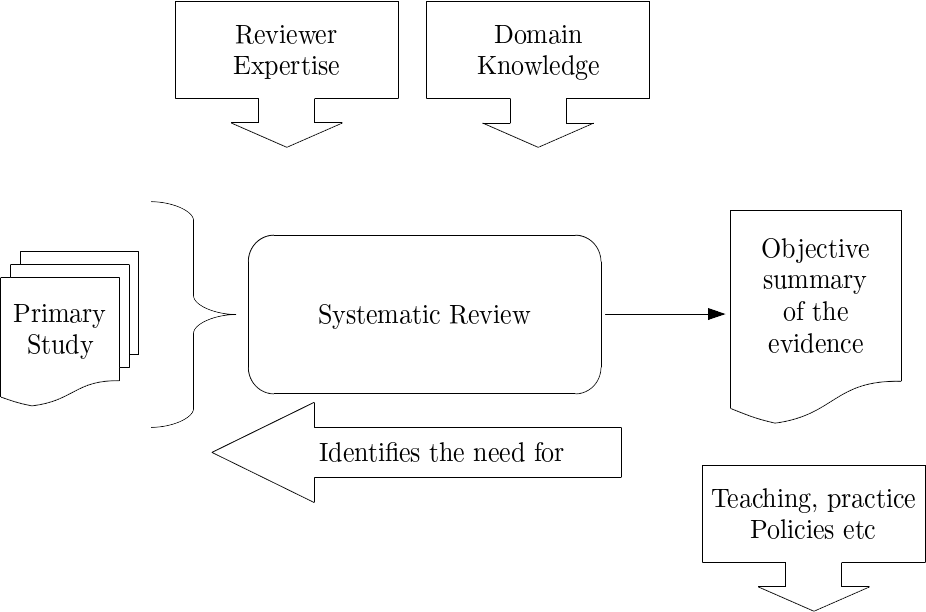
\includegraphics[scale=0.5]{srcontext}
\section{Procedures for a SR}
Phase 1: Plan review
\begin{enumerate}
	\item Specify research question used to create search strings
	\item Develop review protocol (plan)
	\item Validate protocol, which may include prototyping search strings
\end{enumerate}
Phase 2: Conduct review
\begin{enumerate}
	\item Execute search strategy, strings, sources, bounding dates etc
	\item Select primary studies, title, abstract, full paper
	\item Assess study quality
	\item Data extraction
	\item Synthesise the data to answer the research question
\end{enumerate}
Phase 3: Document the outcomes
\end{document}